%%%%%%%%%%%%%%%%%%%% book.tex %%%%%%%%%%%%%%%%%%%%%%%%%%%%%
%
% sample root file for the chapters of your "monograph"
%
% Use this file as a template for your own input.
%
%%%%%%%%%%%%%%%% Springer-Verlag %%%%%%%%%%%%%%%%%%%%%%%%%%


% RECOMMENDED %%%%%%%%%%%%%%%%%%%%%%%%%%%%%%%%%%%%%%%%%%%%%%%%%%%
\documentclass[envcountsame,envcountchap]{svmono}
%\documentclass[envcountsame,envcountchap]{svmono}

% choose options for [] as required from the list
% in the Reference Guide, Sect. 2.2

\usepackage{makeidx}         % allows index generation
\usepackage{graphicx}        % standard LaTeX graphics tool
\usepackage{amsmath,amssymb}         % matrices
\usepackage{enumerate}
\usepackage{dynkin-diagrams}
\usepackage{pstricks}
\usepackage{pdfpages}
\usepackage{svg}

                             % when including figure files
\usepackage{multicol}        % used for the two-column index
\usepackage[bottom]{footmisc}% places footnotes at page bottom
% etc.
% see the list of further useful packages
% in the Reference Guide, Sects. 2.3, 3.1-3.3


\DeclareMathOperator{\End}{End}
\DeclareMathOperator{\Aut}{Aut}
\DeclareMathOperator{\Hom}{Hom}
\DeclareMathOperator{\support}{supp}


% NEW COMMANDS

%It is standard in Latex to write "macros" which are shorthand for an entire series of instructions. Here are some examples

%Number sets
\newcommand{\N}{\mathbb N}
%So typing \N produces the correct mathematical symbol for the natural numbers
\newcommand{\Z}{\mathbb Z}
\newcommand{\Q}{\mathbb Q}
\newcommand{\R}{\mathbb R}
\newcommand{\C}{\mathbb C}
\newcommand{\K}{\mathbb K}
%notations quelquonques
\newcommand{\tg}[1]{\textbf{#1}}
\newcommand{\ub}[1]{\overline{#1}}

%notations des objets simples
\newcommand{\es}{\emptyset}
\newcommand{\nes}{$\not= \emptyset$}
\newcommand{\sub}{\subset}
\newcommand{\norm}[2]{\lVert #1 \lVert_{#2}}
\newcommand{\vect}[2]{(#1_1,#1_2, \dots, #1_#2)}
\newcommand{\modu}[1]{\lvert#1\lvert}
\newcommand{\B}[3]{B_{#1}\big(#2,#3\big[}
%notations mathématiques
\newcommand{\lb}{\lbrack}
\newcommand{\rb}{\rbrack}
\newcommand{\lv}{\lVert}
%limits and sum
\newcommand{\s}[2]{\sum\limits_{#1}^{#2}}
\newcommand{\li}[2]{\xrightarrow[#1\rightarrow#2]{}}
\newcommand{\lis}[1]{\xrightarrow[n\rightarrow+\infty]{#1}}
\newcommand{\lif}[1]{\xrightharpoonup[n\rightarrow+\infty]{#1}}
\newcommand{\lic}[3]{\xrightarrow[#1\rightarrow#2]{#3}}

\newcommand{\bcup}[2]{\bigcup\limits_{#1}^{#2}}
\newcommand{\bcap}[2]{\bigcap\limits_{#1}^{#2}}

\newcommand{\inv}[1]{\frac{1}{#1}}
\newcommand{\prods}[2]{\langle\qq #1\qq,\qq#2\qq\rangle}

\newcommand{\restr}[2]{#1_{\mkern 2mu \vrule height 2ex\mkern2mu #2} }
\newcommand{\quot}[2]{{\raisebox{.2em}{$#1$}\left/\raisebox{-.2em}{$#2$}\right.}}
\newcommand{\limite}[2]{\underset{#1\rightarrow#2}{\text{lim}}}
\newcommand{\espp}[2]{Ker\big(u-{#1} Id_{#2}\big)}
\newcommand{\fct}[4]{\qq:\qq #1\qq\longrightarrow\qq #2\qq :\qq #3\qq \mapsto\qq #4}

\newcommand{\lam}{\lambda}
\newcommand{\q}{\quad}
\newcommand{\qq}{\text{ }}

\newcommand{\liste}[2]{#1_1, #1_2,..,#1_{#2}}

\newcommand{\maxx}[1]{\underset{#1}{\text{max}}}
\newcommand{\minn}[1]{\underset{#1}{\text{min}}}
\newcommand{\supp}[1]{\underset{#1}{\text{sup}}}
\newcommand{\inff}[1]{\underset{#1}{\text{inf}}}

\newcommand{\fctt}[2]{\qq:\qq#1\qq\rightarrow\qq#2}
\newcommand{\liminff}[1]{\underset{#1\rightarrow+\infty}{\text{liminf}}}
\newcommand{\limsupp}[1]{\underset{#1\rightarrow+\infty}{\text{limsup}}}

\newcommand{\adh}[2]{\text{Adh}_{#1}\big(#2\big)}
\newcommand{\wed}[3]{#1_#2\wedge\dots \wedge #1_#3}


\makeindex             % used for the subject index
                       % please use the style svind.ist with
                       % your makeindex program


%%%%%%%%%%%%%%%%%%%%%%%%%%%%%%%%%%%%%%%%%%%%%%%%%%%%%%%%%%%%%%%%%%%%%

\begin{document}

\author{MATH-F-427 students}
\title{Coxeter groups}
\subtitle{Course notes}
\maketitle

\frontmatter%%%%%%%%%%%%%%%%%%%%%%%%%%%%%%%%%%%%%%%%%%%%%%%%%%%%%%

\tableofcontents


\mainmatter%%%%%%%%%%%%%%%%%%%%%%%%%%%%%%%%%%%%%%%%%%%%%%%%%%%%%%%
\part{Coxeter groups}
\chapter{Preliminaries}

This chapter is based on the first chapter of \cite{magnusCombinatorialGroupTheory2004}. This constitutes a recap of what groups are and how they are generated.\\

We recall that a group $(G,\cdot)$ is a non-empty set $G$ of elements equipped with a binary operation $\cdot\qq :\qq  G \times G \rightarrow G$ for which the next properties are satisfied :

\begin{itemize}
  \item \textbf{Associativity:} The operation $\cdot$ is associative, which means that for any elements $a,b,c \in G$ :
    $$(ab)c = a(bc)$$

  \item \textbf{Identity element:} There exists an element of $G$ noted $e$ for which :

  $$a\cdot e = e\cdot a = a$$

  \item \textbf{Inverse element:} For any $a \in G$ there exists an \textit{element} $a^{-1}$ for which :
  $$ a\cdot a^{-1} = a^{-1} \cdot a = e $$
\end{itemize}

There are a lot of ways to define groups. However, the two most ``common" ways in the everyday mathematics is to consider set of \textit{symmetries} or to give an explicit presentation of the group in terms of generators and relations.

\section{Symmetric groups}

\begin{definition}[Symmetric group]
The symmetric group on the set $M$ is the group whose elements are permutations of the elements of $M$ and its operation is the permutation composition. If $M = \{1,\dots, n \}$ we call it $S_n$. \cite{saganSymmetricGroup2001}.
\end{definition}

\begin{proposition}$S_n$ has order $n!$ and every group $G$ of order $n$ is a subgroup of $S_n$.
\end{proposition}

%\subsection{Permutations}

Symmetric groups are based on the behave of permutations and as we explain, there are a very important example of groups since every group is a subgroup of such. The purpose of this subsection is to define the operation on permutations.


\begin{definition}[Two-line notation]
Given a permutation function $\pi$ of ${1,...,n}$, we represent it by listing every elements of the set ${0,...,n}$ in two lines, where the first line represent the starting elements, and the second one, their images through the function $\pi$ :

\begin{equation}
  \begin{pmatrix}
   1 & 2 & 3 & 4 & 5 & \dots & n \\
   \pi(1) & \pi(2) & \pi(3) & \pi(4) & \pi(5) & \ & \pi(n)
 \end{pmatrix}
\end{equation}

\end{definition}


\begin{definition}[Cycle notation]Given $i \in \{1,\dots,n\}$ and $\pi$ a permutation function of $\{1,\dots,n\}$, the elements of the sequence $i, \pi(i), \pi^2(i),\dots$ cannot all be distinct due to the pigeon hole principle. In particular, there must exists a power $p \in \mathbb{N}$ such that $\pi^p(i) = i$. This allow us to write the permutation as a product of cycles of the type :

\begin{equation}
  (i, \pi(i), \pi^2(i), \dots, \pi^{p-1}(i))
\end{equation}
\end{definition}

This means that, given a cycle $(i,j,k)$, the element $i$ is sent to $j$, $j$ is sent to $k$ and $k$ is sent to $i$, cyclically, e.g. the permutation $23145$ of $ \{1,2,3,4,5\}$ can be written with cycle notation as $(1,2,3)(4)(5)$. Remark that every element of the set has to be used.

\section{Presentation of groups}
\label{sec:pres_group}

In this section we show how a group can be defined by generators and relations :

\begin{definition}
  A group can be defined by:
  \begin{equation}
    Gr \cong \langle G | R\rangle
  \end{equation}
where $G = \{a,b,c,\dots\}$ is the set of \emph{generators} and $R = \{A,B,C,\dots\}$ is the set of \emph{relations} such that every $X \in R$ is a word in $(G\cup G^{-1})^*$ satisfying $X = 1$.
\end{definition}

\begin{example}
The dihedral group $D_n$ can be presented in the following way; where $q$ is a rotation and $r$ a reflection :

$$D_n \cong \langle \{q,r\} | \{r^2, q^n, rqrq\} \rangle$$
\end{example}


\chapter{Coxeter groups}

\section{Motivations}
Let us explain the interest and motivation of Coxeter groups by analysing the symmetric group $S_3$, which is a standard example of Coxeter group. This group can be defined in three ways.

\begin{figure}
  \begin {center}
  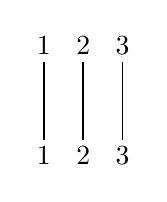
\begin{tikzpicture}
  	% general shift to north east
    \draw (0,1+0.2) node {$1$};
    \draw (0.5,1+0.2) node {$2$};
    \draw (1,1+0.2) node {$3$};
  	\draw[semithick] (0,0) -- (0,1);% first line
  	\draw[semithick] (0.5,0) -- (0.5,1);% second line
  	\draw[semithick] (1,0) -- (1,1);% third line
    \draw (0,-0.2) node {$1$};
    \draw (0.5,-0.2) node {$2$};
    \draw (1,-0.2) node {$3$};
  \end{tikzpicture}

  \caption{The wiring diagram for the permutation $123$.}
  \end{center}
\label{fig:wiring}
\end{figure}

\begin{figure}
  \begin {center}
  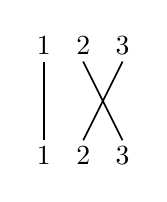
\begin{tikzpicture}
    % general shift to north east
    \draw (0,1+0.2) node {$1$};
    \draw (0.5,1+0.2) node {$2$};
    \draw (1,1+0.2) node {$3$};
    \draw[semithick] (0,0) -- (0,1);% first line
    \draw[semithick] (0.5,0) -- (1,1);% second line
    \draw[semithick] (1,0) -- (0.5,1);% third line
    \draw (0,-0.2) node {$1$};
    \draw (0.5,-0.2) node {$2$};
    \draw (1,-0.2) node {$3$};
  \end{tikzpicture}
  \caption{The wiring diagram for the permutation $132$.}
  \end{center}
\label{fig:wiring_23}
\end{figure}

\begin{figure}
  \begin {center}
  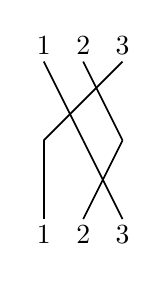
\begin{tikzpicture}
    % general shift to north east
    \draw (0,2+0.2) node {$1$};
    \draw (0.5,2+0.2) node {$2$};
    \draw (1,2+0.2) node {$3$};
    \draw[semithick] (0,0) -- (0,1);% first line
    \draw[semithick] (0,1) -- (1,2);% first line
    \draw[semithick] (0.5,0) -- (1,1);% second line
    \draw[semithick] (0.5,1) -- (0,2);% second line
    \draw[semithick] (1,0) -- (0.5,1);% third line
    \draw[semithick] (1,1) -- (0.5,2);% third line
    \draw (0,-0.2) node {$1$};
    \draw (0.5,-0.2) node {$2$};
    \draw (1,-0.2) node {$3$};
  \end{tikzpicture}

  \caption{The wiring diagram for the permutation composition $132 \circ 231$.}
  \end{center}
\label{fig:wiring_compo}
\end{figure}


\begin{figure}
  \begin{center}
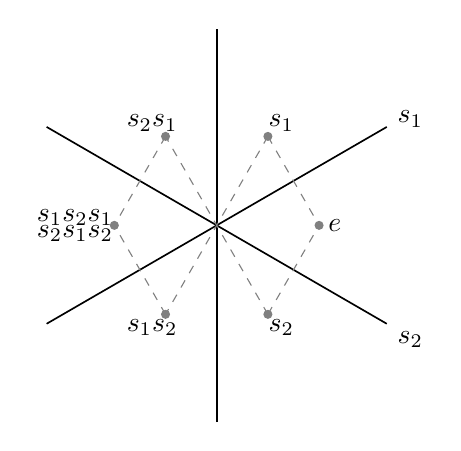
\begin{tikzpicture}
	% general shift to north east
	\draw[semithick] (0,-2.5) -- (0,2.5);% center line
  \draw[semithick] (-2.16,1.25) -- (2.16,-1.25);% first symmetry
  \draw[semithick] (2.16,1.25) -- (-2.16,-1.25);% second symmetry

  \def\offX{0.65}
  \def\offY{1.13}
	\draw[dashed,color=gray] (0+\offX,0+\offY) -- (0.65+\offX,-1.13+\offY);% e to s_1
  \draw[dashed,color=gray] (0+\offX,0-\offY) -- (0.65+\offX,-1.13+\offY);% e to s_2
	\draw[dashed,color=gray] (0+\offX,0+\offY) -- (0-\offX,0-\offY);% s_1 to s_1s_2
  \draw[dashed,color=gray] (0+\offX,0-\offY) -- (0-\offX,0+\offY);% s_2 to s_2s_1
  \draw[dashed,color=gray] (0-\offX,0+\offY) -- (-1.3,0);% s_1s_2 to s_1s_2s_1
  \draw[dashed,color=gray] (0-\offX,0-\offY) -- (-1.3,0);% s_2s_1 to s_2s_1s_2

  \draw [fill=gray, color=gray](1.3,0) circle (0.05);
  \draw [fill=gray, color=gray](-1.3,0) circle (0.05);
  \draw [fill=gray, color=gray](0+\offX,0+\offY) circle (0.05);
  \draw [fill=gray, color=gray](0-\offX,0+\offY) circle (0.05);
  \draw [fill=gray, color=gray](0+\offX,0-\offY) circle (0.05);
  \draw [fill=gray, color=gray](0-\offX,0-\offY) circle (0.05); % s_1s_2

  % axis
  \def\offAx{0.2}
  \draw (2.16+\offAx+0.1,-1.25-\offAx) node {$s_2$};
  \draw (2.16+\offAx+0.1,+1.25+\offAx-0.1) node {$s_1$};

  \draw (1.5,0) node {$e$};
  \draw (-1.8,0+0.1) node {$s_1s_2s_1$};
  \draw (-1.8,0-0.1) node {$s_2s_1s_2$};
  \draw (0+\offX + 0.17,0+\offY + 0.17) node {$s_1$};
  \draw (0+\offX + 0.17,0-\offY - 0.17) node {$s_2$};
  \draw (0-\offX - 0.17,0+\offY + 0.17) node {$s_2s_1$};
  \draw (0-\offX - 0.17,0-\offY - 0.17) node {$s_1s_2$};
\end{tikzpicture}
\end{center}
\caption{Geometrical representation of $S_3$. The grey dotted lines represent the reflection applied between two points.}
\label{fig:geoS3}
\end{figure}

\begin{itemize}
  \item Combinatorially : Given a cyclic permutation, we can represent it as a \emph{wiring diagram}. Some examples of permutations of $123$ are given in the wire diagrams \ref{fig:wiring} and \ref{fig:wiring_23}. Their composition is given by the wire diagram \ref{fig:wiring_compo}.




  \item Algebraically : Presentation of groups as seen in section \ref{sec:pres_group}.
  \begin{equation}\label{equation donnant la form explicite de pi}
  \begin{split}
  S_3 \cong \langle \{s_1, s_2\} | \{ s_1s_2s_1 &= s_2s_1s_2 , s_1^2 = e, s_2^2 = e,\\
   &(s_1s_2)^3 = s_1s_2s_1s_2s_1s_2 = e\} \rangle
  \end{split}
  \end{equation}

  \item Geometrically : We can represent geometrically a coxeter group by reflections. In figure \ref{fig:geoS3} we can see a geometrical representation of $S_3$ where $s_1$ and $s_2$ are the generators of $S_3$ and also reflections on the plane. Notice that $s_1s_2s_1 = s_2s_1s_2$, $s_1^2 = e$ and $s_2^2$; $S_3$ is a coxeter group.
\end{itemize}

\section{Coxeter groups}

In this section we define the notion of Coxeter groups.

\begin{definition} Let $S$ be a finite set.
  A \emph{Coxeter matrix} is a map $m : S\times S \to \{1,2,\dots,\infty\}$ such that:
  \begin{enumerate}
    \item $m(s,s) = 1 \ \ \forall s \in S$
    \item $m(s,s') = m(s', s) \ \ \forall s,s' \in S$
    \item $m(s,s') > 1\ \ \ \text{if}\  s \neq s'$
  \end{enumerate}
\end{definition}

\begin{definition}
  A \emph{coxeter diagram} is a graph where the set of vertices are the elements of $S$ and
  the labelled edges are such that:
  \begin{enumerate}
    \item if $m(s,s') = 2$ : \ \dynkin[labels={s},label macro/.code={#1}]{A}{1}
                      \dynkin[labels={s'},label macro/.code={#1}]{A}{1}
    \item if $m(s,s') = 3$ :   \dynkin[labels={s,s'},label macro/.code={#1}]{A}{2}
    \item if $m(s,s') \geq 4$ : \dynkin[labels={s,s'},label macro/.code={#1}]{A}{2} where the label of the edge is $m(s,s')$.
  \end{enumerate}
where in this definition, $m$ is the Coxeter matrix.
\end{definition}

\begin{example}
	If we have a Coxeter matrix $m$:
    \begin{equation}
      m =
    \begin{bmatrix}
    1 & 3 & 2\\
    3 & 1 & 4\\
    2 & 4 & 1\\
    \end{bmatrix}
    \end{equation}
where the line or column $i$ corresponds to the element $s_i \in S$. Then the related Coxeter diagram can be drawn like this:

  \center{\dynkin[Coxeter, labels={s_1, s_2, s_3}]{B}{3}}
\end{example}

Given the definition of $m$, we can now define formally a coxeter group.

\begin{definition}
A \emph{coxeter group} is a group with the following presentation:

\begin{equation}
  \langle S\  |\{  (ss')^{m(s,s')} = e, \forall s, s' \in S\} \rangle
\end{equation}
where $S$ si a set and $m$ the coxeter matrix with $m(s,s') < \infty$.

\end{definition}

\begin{example}
  The symmetric group $S_n$ is a Coxeter group that can be represented by the following Coxeter diagram:
  \begin{center}
    \dynkin[Coxeter, labels={s_1, s_2, s_{n-1}, s_n}, edge length=.50cm]{A}{}
  \end{center}
In fact, for every $i < n$, we have that $s_is_{i+1}s_is_{i+1} = e$, so $(s_is_{i+1})^2 = e$, which means that
  $m(s_i, s_{i+1}) = 2$ for every $i < n$.
\end{example}

\begin{definition}
  The pair $(W,S)$ is a Coxeter system where $W$ is a Coxeter group and $S$ a group of generators.
\end{definition}

\begin{figure}
  \begin {center}
  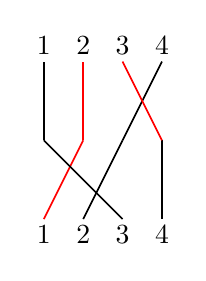
\begin{tikzpicture}
    \draw (0,2+0.2) node {$1$};
    \draw (0.5,2+0.2) node {$2$};
    \draw (1,2+0.2) node {$3$};
    \draw (1.5,2+0.2) node {$4$};
    \draw[semithick, color=red] (0,0) -- (0.5,1);% first line
    \draw[semithick, color=red] (0.5,1) -- (0.5,2);% first line
    \draw[semithick] (0.5,0) -- (1,1);% second line
    \draw[semithick] (0,1) -- (0,2);% second line
    \draw[semithick] (1,0) -- (0,1);% third line
    \draw[semithick] (1,1) -- (1.5,2);% third line
    \draw[semithick] (1.5,0) -- (1.5,1);% fourth line
    \draw[semithick, color=red] (1.5,1) -- (1,2);% fourth line
    \draw (0,-0.2) node {$1$};
    \draw (0.5,-0.2) node {$2$};
    \draw (1,-0.2) node {$3$};
    \draw (1.5,-0.2) node {$4$};
  \end{tikzpicture}
  \caption{The wiring diagram for the permutation  $3\bar{1}24 \circ 1\bar{2}\bar{4}3$. You can see that there is a permutation that changes its sign two times.}
  \end{center}
\label{fig:wiring_snB}
\end{figure}

We introduce the hyperoctahedral group $S_n^B$ as being the group of signed permutations of $\big[n\big] := \{1, 2, \dots, n\}$. The group set is $\{1,2,\dots,m,\bar{1}, \bar{2},\dots, \bar{n}\}$. We have a new generator $t$, that will change the sign of an element. In figure \ref{fig:wiring_snB} we can see an example of permutation within this group. This is a Coxeter group and its diagram is:

\begin{center}
  \dynkin[Coxeter, labels={s_n, s_{n-1}, s_{n-2},s_2,s_1, t}, edge length=.50cm, gonality=n ]{B}{}
\end{center}

Given a Coxeter system $(W,S)$, we can define $T := \{wsw^{-1} |\ s\in S, w \in W\} \subseteq W$ where $s$ are simple reflections.

\begin{definition}
  Given $W \to S_T^B : w \to \pi_w$, $t\in T$ and $s\in S$:

  \begin{equation}
    \pi_s(t) := \left \{
    \begin{array}{c @{} c}
        -s \quad &\text{if } t = s \\
        sts \quad &\text{if } t \neq s \\
    \end{array}\right.
  \end{equation}
\end{definition}
This application is a bijection because its inverse is itself ($\pi_s(\pi_s(s)) = s$):

\begin{equation}
  \pi(\pi_s(t)) = \left \{
  \begin{array}{c @{} c}
      \pi_s(-s) \quad &\text{if } t = s \\
      \pi_s(tsts) \quad &\text{if } t \neq s \\
  \end{array}\right.
\end{equation}
We clearly see that $\pi_s(sts) = s(sts)s = t$ and $\pi_s(-s) = -\pi_s(s) = -s$.

%\begin{equation}

%\end{equation}


	\begin{theorem}
		The application $\pi$ that we defined on the set of generators $S$ of the Coxeter system $(W,S)$, extends uniquely to an injective homomorphism $\pi\fctt{W}{S^B_T}$
	\end{theorem}
	\begin{proof}
		First of all, we need to show that the extension of $\pi$ is well defined. It was clear, due to the definition of $\pi$ on $S$ that for every $s\in S$, the application $\pi_s\in S^B_T$. Indeed, for every $t\in T$ we had that $\pi_s(t)\in T\cup \ub{T}$ and we had that $\pi_s$ defined a bijection on $T\cup \ub{T}$. Now, we need to check that its extension on all of $W$ is still well defined. We need to check 2 things. First, we need to check that $\forall w\in W$ the application $\pi_w\in S_T^B$. But, since we extended $\pi$ from $S$ to $W$ to be a group morphism, we know that $\pi_w$ is by definition the composition of $\pi_s$ for some $s\in S$ and thus is an element of $S_T^B$. Secondly, we need to check that this application $\pi_w$ does not depend on the writing of $w\in W$. To this aim, let us take $t\in T$ and let $w=s_1s_2..s_k$ for some $s_i\in S$ (this is the form of every element of $W$ since $s_i=s_i^{-1}$ for all $i$). Since, we want $\pi$ to be a homomorphism, we have that :
		\begin{equation}\label{equation donnant la form explicite de pi}
		\begin{split}
		\pi_w(t)\qq&=\qq \pi_{s_1}\circ\pi_{s_2}\circ ... \circ \pi_{s_k}(t)\\
		&=\qq \pi_{s_1}\circ\pi_{s_2}\circ ... \circ \pi_{s_{k-1}}(\pm s_kts_k)\q\q\\
		& \q\q (\mbox{with }-\mbox{ iff }s_kts_k=s_k\iff t=s_k)\\
		&=\qq \pi_{s_1}\circ\pi_{s_2}\circ ... \circ \pi_{s_{k-2}}(\pm\pm s_{k-1}s_kts_ks_{k-1})\q\q\\
		& \q\q(\mbox{with }-\mbox{ iff }s_{k-1}s_kts_ks_{k-1}=s_{k-1}\iff t=s_ks_{k-1}s_k)\\
		&=\qq \pi_{s_1}\circ\pi_{s_2}\circ ... \circ \pi_{s_{k-3}}(\pm\pm\pm s_{k-2}s_{k-1}s_kts_ks_{k-1}s_{k-2})\q\q \\
		&\q\q (\mbox{with }-\mbox{ iff }s_{k-1}s_kts_ks_{k-1}=s_{k-1}s_{k-2}\iff t=s_ks_{k-1}s_{k-2}s_{k-1}s_k)\\
		&=\q\q \q\vdots\q\q \q\vdots\q\q \q\vdots\q\q \q\vdots\q\q \q\vdots\q\q \q\vdots\q\q \q\vdots\q\q \q\vdots\q\q \q\vdots\\
		&=\qq \pm\pm \dots \pm s_1s_2...s_kts_ks_{k-1}... s_1\q\q\\
		& \q\q (\mbox{with }-\mbox{ iff }s_1...s_{k-1}s_kts_ks_{k-1}...s_1=s_{1}\iff t=s_k...s_2s_1s_2...s_k)\\
		&=\mbox{sgn}_w(t)\qq wtw^{-1}
		\end{split}
		\end{equation}
		where the function $\mbox{sgn}_w(t)$ is a sign function counting the number of times we have an index $l\in \{1,2,...k\}$ such that $t=s_k...s_{l-1}s_l s_{l-1}...s_k$. Namely :
		\begin{equation}
		 \mbox{sgn}_w(t)\qq=\qq (-1)^{\# \{1\leq l\leq k\qq :\qq t=s_k...s_{l-1}s_l s_{l-1}...s_k\}}
		\end{equation}
		As we will show just after this sign function does not depend of the writing of $w\in W$ in the Coxeter system $(W,S)$.

		But first, let us get some intuition about what this sign function is counting with a visual representation that we have seen before in the chapter: wiring diagrams. In figure \ref{fig:wiring_sign} you can find an example for $S_n$.
		\begin{figure}

		  \begin {center}
		  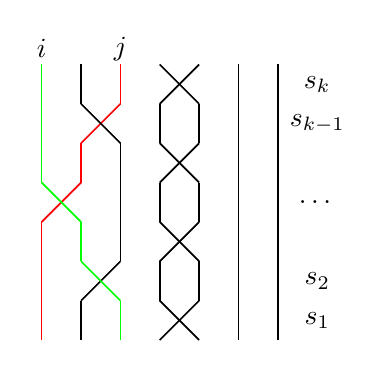
\begin{tikzpicture}

				\def\xa{0}
				\def\xb{0.5}
				\def\xc{1}
				\def\xd{1.5}
				\def\xe{2}
				\def\xf{2.5}
				\def\xg{3}

				%first level
				\draw[semithick, color=red] (\xa,0) -- (\xa,0.5);
				\draw[semithick] (\xb,0) -- (\xb,0.5);
				\draw[semithick, color=green] (\xc,0) -- (\xc,0.5);
				\draw[semithick] (\xd,0) -- (\xe,0.5);
				\draw[semithick] (\xe,0) -- (\xd,0.5);
				\draw[semithick] (\xf,0) -- (\xf,0.5);
				\draw[semithick] (\xg,0) -- (\xg,0.5);

				%second level
				\draw[semithick, color=red] (\xa,0.5) -- (\xa,1);
				\draw[semithick] (\xb,0.5) -- (\xc,1);
				\draw[semithick, color=green] (\xc,0.5) -- (\xb,1);
				\draw[semithick] (\xd,0.5) -- (\xd,1);
				\draw[semithick] (\xe,0.5) -- (\xe,1);
				\draw[semithick] (\xf,0.5) -- (\xf,1);
				\draw[semithick] (\xg,0.5) -- (\xg,1);

				%third level
				\draw[semithick, color=red] (\xa,1) -- (\xa,1.5);
				\draw[semithick, color=green] (\xb,1) -- (\xb,1.5);
				\draw[semithick] (\xc,1) -- (\xc,1.5);
				\draw[semithick] (\xd,1) -- (\xe,1.5);
				\draw[semithick] (\xe,1) -- (\xd,1.5);
				\draw[semithick] (\xf,1) -- (\xf,1.5);
				\draw[semithick] (\xg,1) -- (\xg,1.5);

				%fourth level
				\draw[semithick, color=red] (\xa,1.5) -- (\xb,2);
				\draw[semithick, color=green] (\xb,1.5) -- (\xa,2);
				\draw[semithick] (\xc,1.5) -- (\xc,2);
				\draw[semithick] (\xd,1.5) -- (\xd,2);
				\draw[semithick] (\xe,1.5) -- (\xe,2);
				\draw[semithick] (\xf,1.5) -- (\xf,2);
				\draw[semithick] (\xg,1.5) -- (\xg,2);

				%fifth level
				\draw[semithick, color=green] (\xa,2) -- (\xa,2.5);
				\draw[semithick, color=red] (\xb,2) -- (\xb,2.5);
				\draw[semithick] (\xc,2) -- (\xc,2.5);
				\draw[semithick] (\xd,2) -- (\xe,2.5);
				\draw[semithick] (\xe,2) -- (\xd,2.5);
				\draw[semithick] (\xf,2) -- (\xf,2.5);
				\draw[semithick] (\xg,2) -- (\xg,2.5);

				%sixth level
				\draw[semithick, color=green] (\xa,2.5) -- (\xa,3);
				\draw[semithick, color=red] (\xb,2.5) -- (\xc,3);
				\draw[semithick] (\xc,2.5) -- (\xb,3);
				\draw[semithick] (\xd,2.5) -- (\xd,3);
				\draw[semithick] (\xe,2.5) -- (\xe,3);
				\draw[semithick] (\xf,2.5) -- (\xf,3);
				\draw[semithick] (\xg,2.5) -- (\xg,3);

				%seventh level
				\draw[semithick, color=green] (\xa,3) -- (\xa,3.5);
				\draw[semithick] (\xb,3) -- (\xb,3.5);
				\draw[semithick, color=red] (\xc,3) -- (\xc,3.5);
				\draw[semithick] (\xd,3) -- (\xe,3.5);
				\draw[semithick] (\xe,3) -- (\xd,3.5);
				\draw[semithick] (\xf,3) -- (\xf,3.5);
				\draw[semithick] (\xg,3) -- (\xg,3.5);

				\draw (\xa,3.7) node {$i$};
		   	\draw (\xc,3.7) node {$j$};

				\draw (\xg+0.5,3.25) node {$s_k$};
				\draw (\xg+0.5,2.75) node {$s_{k-1}$};
				\draw (\xg+0.5,1.75) node {\ldots};
				\draw (\xg+0.5,0.75) node {$s_2$};
				\draw (\xg+0.5,0.25) node {$s_1$};

		  \end{tikzpicture}
		  \caption{ A wiring diagram for a word $w \in W$ of the coxeter group $S_n$. You can see that $sgn_w(t)$ with $t = (i,j)$ equals 1 because there is only one crossing between the wires that begin at $i$ and $j$.}
		  \end{center}
		\label{fig:wiring_sign}
		\end{figure}



		We are now going to use equation \ref{equation donnant la form explicite de pi} to prove that $\pi$ is a well defined homomorphism which is equivalent to show that the sign function does not depend on the writing of $w\in W$ in the Coxeter system $(W,S)$. It suffices to show that all the relations we had in $(W,S)$ are satisfied by their image in $S^B_T$. I.e. let us take $s,s'\in S$, we want to show that :
		\begin{equation}\label{equation provant que les relations sont preserves par pi}
		(\pi_s\circ \pi_{s'})^{m(s,s')}\qq=\qq \mbox{Id}_{S^B_T}
		\end{equation}
		Since $(ss')^{-1}=s's$, equation \ref{equation donnant la form explicite de pi} gives for all $t\in T$ :
		\begin{equation}
		(\pi_s\circ \pi_{s'})^{m(s,s')}(t)\qq=\qq \pm\qq (ss')^{m(s,s')}t(s's)^{m(s,s')}\qq=\qq \pm \qq et e\qq=\qq\pm \qq  t
		\end{equation}
		But the sign must be $+$ as here, $w=(ss')^{m(s,s')}$ and therefore we look at :
		\begin{equation}
		{\# \{1\leq l\leq m(s,s') \qq :\qq t=\underset{2l-1 \mbox{ characters}}{\underbrace{s'ss'...s'ss'}}\}}
		\end{equation}
		Which must be even. Indeed, if for some $l\leq m(s,s')/2$ we have :
		\begin{itemize}
			\item if $ m(s,s')$ is even :
			\begin{equation}
			t\qq=\qq \underset{2l-1 \mbox{ characters}}{\underbrace{s'ss'...s'ss'}}\qq=\qq\underset{2l-1 + m(s,s') \mbox{ characters}}{\underbrace{s'ss'...s'ss'}}\qq=\qq \underset{2(l+m(s,s')/2)-1 \mbox{ characters}}{\underbrace{s'ss'...s'ss'}}
			\end{equation}
			\item  if $ m(s,s')$ is odd :
			\begin{equation}
			t\qq=\qq \underset{2l-1 \mbox{ characters}}{\underbrace{s'ss'...s'ss'}}\qq=\qq\underset{2l-1 +m(s,s') \mbox{ characters}}{\underbrace{s'ss'...s'ss'}}\qq=\qq \underset{2((m(s,s')-1)/2+l)+1 \mbox{ characters}}{\underbrace{s'ss'...s'ss'}}
			\end{equation}
		\end{itemize}
	This shows that if one index is counted below $m(s,s')/2$ then there exists an other index counted strictly upper than $m(s,s')/2$ and vis versa. Thus the set must be even and the sign must be $+$. Therefore, equation \eqref{equation provant que les relations sont preserves par pi}, is proved and we $\pi$ is a well defined morphism.

	It remains to show that the extension of $\pi$ is injective. Let $u,v\in W$ be such that $\pi_u=\pi_v$ then, we have that :
	\begin{equation}
	\pi_{uv^{-1}}\qq=\qq \pi_u\circ \pi_{v^{-1}}\qq=\qq \mbox{Id}_{S_T^B}\qq=\qq  \pi_e
	\end{equation}
	Thus, we just need to show that if $w\in W$ is such that $\pi_w=\pi_e$ then $w=e$ to prove the injectivity of $\pi$. Now, let us take $w\in W$ such that $\pi_w=\pi_e$ and let us suppose absurdly that $w\not=e$ then, there exists $k\geq 1$ such that $w=s_1...s_k$ is the shorter way possible to write $w\in W$ then (meaning that $k$ is the smallest possible) :
	\begin{equation}\label{equation pour la contradiction par signe de sk}
	\begin{split}
		s_k\qq=\qq\pi_e(s_k)\qq&=\qq \pi_w(s_k)\qq =\qq\mbox{sgn}_w(s_k)\qq s_1...s_{k-1}s_ks_ks_ks_{k-1}...s_1\qq\\
		&=\qq\mbox{sgn}_w(s_k)\qq s_1...s_{k-1}s_ks_{k-1}...s_1
	\end{split}
	\end{equation}
	But $\mbox{sgn}_w(s_k)=-1$ because :
	\begin{equation}
	\{1\leq l\leq k\qq :\qq t=s_k...s_{l-1}s_l s_{l-1}...s_k\}\qq=\qq \{k\}
	\end{equation}
	Indeed, for $l=k$ we have $s_k=s_k$. But if $l\not=k$ and if we had :
	\begin{equation}
	s_k=\qq s_k..s_l..s_k
	\end{equation}
	Then we would have :
	\begin{equation}
	s_{l-1}...s_ks_k\qq=\qq s_l...s_k
	\end{equation}
	Therefore, we would have a contradiction with the minimality of $k$ since :
	\begin{equation}
	\begin{split}
	w&=s_1...s_ls_{l-1}s_l...s_k\qq\\
	&=\qq s_1...s_{l-1}s_{l-1}...s_ks_k\qq\\
	&=\qq s_1..s_{l-2}s_{l+1}...s_{k-1}\qq\\
	&=\qq s_1...s_{l-2}s_{l+11}...s_{k-1}
	\end{split}
	\end{equation}
	which is a shorter way to write $w$. Therefore, we have that $\mbox{sgn}_w(s_k)=-1$ and thus equation \ref{equation pour la contradiction par signe de sk} gives :
	\begin{equation}
			s_k\qq=\qq -\qq  s_1...s_{k-1}s_ks_{k-1}...s_1
	\end{equation}
	which is a contradiction due to the presence of a sign.\qed
	\end{proof}


	We are now going to define the notions of \tg{parity} and \tg{length} of an element in a Coxeter group.
	\begin{definition}
		Let $(W,S)$ be a Coxeter system, and let $w\in W$, then we say that $w=s_1...s_k$ $(s_l\in S)$ is :
		\begin{itemize}
			\item \tg{even} when $k$ is even.
			\item \tg{odd} when $k$ is odd.
		\end{itemize}
	This is what we call the \tg{parity} of $w\in W$.
	\end{definition}
\begin{remark}
	As all the relations of a Coxeter group involve a pair number of $s\in S$ we see that the parity of an element $w\in W$ doesn't depend on its writing in $W$.
\end{remark}
The set of even elements of a Coxeter system $(W,S)$ is a subgroup of $W$ called the \tg{alternating} subgroup.
\begin{remark}
	When $S_n$ is seen as a Coxeter group with $S=\{s_1...s_{n-1}\}$ and the Coxeter matrix $m(s_i,s_{i+1})=3$ and $m(s,s')=2$ for every other couple $(s,s')\not=(s,s)$ see that the two notions of alternating group coincide.
\end{remark}
\begin{definition}
	Let $(W,S)$ be a Coxeter system, the \tg{length} $l(w)$ of an element $w\in W$ is defined as the smallest integer $k\in \N$ such that there exists $s_1,...,s_k\in S$ with $w=s_1...s_k$.
\end{definition}
The purpose of what follows is to prove the following theorem :
\begin{theorem}\label{theorem sur le calcul des longueurs}
	Let $(W,S)$ be a Coxeter system, and let $w\in W$ then :
	\begin{equation}
	l(w)\qq=\qq \#\{t\in T\qq :\qq \mbox{sgn}_{w^{-1}}(t)=-1\}
	\end{equation}
\end{theorem}
\begin{example}
	In the case where $W=S_n$ with the common representation, $l(w)$ is exactly the number of inversions of $w^{-1}$ which is exactly the same as the number of inversions of $w$ itself.
\end{example}
Before proving this theorem, we focus our attention on some lemma :
\begin{lemma}\label{le lemme de la longueur de tw}
	Let $(W,S)$ be a Coxeter system and let $w\in W$, $t\in T$ then :
	\begin{equation}
	\mbox{sgn}_{w^{-1}}(t)=-1\q \iff \q l(tw)\qq<\qq l(w)
	\end{equation}
\end{lemma}
\begin{proof}
	Let's suppose that $\mbox{sgn}_{w^{-1}}(t)=-1$ and let $w=s_1...s_k$ with $k=l(w)$ then $w^{-1}=s_k...s_1$. We know that there must exist some $1\leq l\leq k$ such that $t=s_1...s_l..s_1$ but then :
	\begin{equation}
	\begin{split}
	tw\qq&=\qq s_1s_2...s_l...s_1\qq q_1s_2...s_ls_{l+1}...s_k\\
	&=\qq s_1s_2...s_{l-1}s_{l+1}...s_k\\
	&=\qq s_1s_2...\hat{s_l}...s_k
	\end{split}
	\end{equation}
	from which we conclude that $l(tw)\leq k-1\qq <\qq k=l(w)$ and the first implication is proven.\\
	Conversely, let's suppose that $l(tw)<l(w)$ then, as $tt=e$ we have that :
	\begin{equation}
	l(tw)\qq <\qq l(ttw)\qq \Rightarrow l(ttw)\not<l(tw)
	\end{equation}
	Therefore, the first implication that we already proved, gives us by taking $\tilde{w=tw}$ that :
	\begin{equation}
	\mbox{sgn}_{w^{-1}t}(t)=+1
	\end{equation}
	Thus,
	\begin{equation}
	\pi_{(tw)^{-1}}(t)\qq=\qq +1 \qq (tw)^{-1}\qq t\qq(tw)\qq=\qq w^{-1}tw
	\end{equation}
	But, by the fact that $\pi$ is a morphism we have that :
	\begin{equation}\label{pi est un homo}
	\pi_{(tw)^{-1}}\qq=\qq\pi_{w^{-1}t}\qq=\qq =\pi_{w^{-1}}\circ\pi_t
	\end{equation}
	Now let's remark that $\forall t\in T$ we have that :
	\begin{equation}
	\pi_t(t)\qq=\qq \mbox{sgn}_t(t)\qq ttt\qq=\qq -t
	\end{equation}
	Indeed, let's write $t=s_1...s_kss_k...s_1$ for a $k$ that is minimal. Then it is clear that :
	\begin{equation}\label{le signe de t de t}
	\{1\leq l\leq 2k+1\qq :\qq t=s_1...s_{l-1}s_l s_{l-1}...s_1\}\qq=\qq \{k+1\}
	\end{equation}
	as by the minimality, it can't be true for $l\leq k$ that $t=s_1...s_{l-1}s_l s_{l-1}...s_1$ and as if it is true for some $l= k+1+l'$ with $l'>0$ we have that
	\begin{equation}
	t\qq=\qq s_1s_2...s_kss_k...s_{k-l'+1}s_{k-l'}s_{k-l'+1}...s_kss_k...s_2s_1
	\end{equation}
	Therefore, by multiplying both sides by $s_1s_2...s_ks$ from the right and by $ss_k...s_2s_1$ from the left, we obtain that :
	\begin{equation}
	s\qq=\qq s_k...s_{k-l'+1}s_{k-l'}s_{k-l'+1}...s_k
	\end{equation}
	Therefore, by replacing $s$ in $t$ we have that :
	\begin{equation}
	t\qq=\qq s_1...s_kss_k...s_1\qq=\qq s_1...s_ks_k...s_{k-l'+1}s_{k-l'}s_{k-l'+1}...s_ks_k...s_1\qq=\qq s_1...s_{k-l'}...s_1
	\end{equation}
	which again contradicts the minimality of $k$. Therefore, the equality \eqref{le signe de t de t} is verified and we have that :
	\begin{equation}
	\pi_t(t)\qq=\qq -t
	\end{equation}
	And by computing equality \eqref{pi est un homo} on $t$ we obtain that :
	\begin{equation}
	\begin{split}
	\pi_{(tw)^{-1}}(t)\qq&=\qq \pi_{w^{-1}}\pi_t(t)\qq\\
	&=\qq \pi_{w^{-1}}(-t)\qq\\
	&=\qq -\qq \pi_{w^{-1}}(t)\\
	&=\qq -\mbox{sgn}_{w^{-1}}(t)\qq w^{-1}tw
	\end{split}
	\end{equation}
	And we finally conclude that $\mbox{sgn}_{w^{-1}}(t)=-1$.\qed
\end{proof}

As a Corollary we have the following lemma :
\begin{lemma}[Exchange property]
Let $(W,S)$ be a Coxeter system and let $w=s_1s-2...s_k\in W$ and $t\in T$, then, if $l(tw)<l(w)$ then, there exists some $1\leq l\leq k$ such that :
	\begin{equation}
	tw\qq=\qq s_1s_2...\hat{s_l}... s_k
	\end{equation}
\end{lemma}
\begin{proof}
	By the previous lemma, we know that $\mbox{sgn}_{w^{-1}}t\qq=\qq -1$. Therefore, we know there exists a $1\leq l\leq k$ such that $tw\qq=\qq s_1s_2...\hat{s_l}... s_k$.\qed
\end{proof}
\begin{lemma}
	Let $(W,S)$ be a Coxeter system and let $w=s_1s_2...s_k\in W$, with $k=l(w)$ and let's take $t\in T$. Then, the following are equivalent :
	\begin{enumerate}
		\item $l(tw)<l(w)$
		\item $tw\qq=\qq s_1...\hat{s_l}...s_1$ for some $1\leq l\leq k$
		\item $t=s_1...s_l...s_1$ for some $1\leq l\leq k$
	\end{enumerate}
Moreover, such an $l$ is uniquely determined.
\end{lemma}
\begin{proof}
	By Lemma \ref{le lemme de la longueur de tw} we already know that $(1)$ implies $(2)$. Furthermore, the equivalence between $(2)$ and $(3)$ is a tautology. Let us prove that $(2)$ implies $(1)$. Indeed, if $tw\qq=\qq s_1...\hat{s_l}...s_1$ for some $1\leq l\leq k$ then :
	\begin{equation}
	l(tw)\qq \leq \qq k+1\qq <\qq k \qq=\qq l(w)
	\end{equation}
	which is $(1)$. It remains to show that this $l$ appearing in property $(2)$ and $(3)$ is unique under the hypothesis that $k=l(w)$. Let us define $t_i=s_1s_2...s_i...s_1$ for all $1\leq i\leq k$. Then, we want to show that  $t_i\not=t_j$ for every $i\not=j$. Let's reason by absurd and suppose the contrary. Therefore, there exists $i<j$ such that $t_i=t_j$. Then,
	\begin{equation}
	\begin{split}
	w\qq&=\qq t_it_j\qq w\\
	&=\qq t_is_1...\hat{s_j}...s_k\\
	&=\qq s_1...\hat{s_i}...\hat{s_j}...s_k
	\end{split}
	\end{equation}
	as $i$ was less than $j$. But this is a contradiction with the exchange property applied for $t=t_it_j$. Therefore we needed that $t_i\not=t_j$ for every $i\not=j$. In particular $l$ must be unique.
	\qed
\end{proof}
With all those lemma, we are now ready to prove theorem \ref{theorem sur le calcul des longueurs}.
\begin{proof}
	Let $w=s_1s_2...s_k$ with $k=l(w)$, then $w^{-1}=s_k...s_1$ and due to the previous lemma, we know that :
	\begin{equation}
	\begin{split}
		\#\{t\in T\qq :\qq \mbox{sgn}_{w^{-1}}(t)=-1\}\qq\q\q\q\q\q\q\q \\
		=\qq \# \{t\in T\qq:\qq t=s_1...s_i...s_k\qq \mbox{for some }1\leq l\leq k\}\qq=\qq k\qq =l(w)
	\end{split}
	\end{equation}
	as every of the $t_i=s_1...s_i...s_1$ are different from each other. \qed
\end{proof}


The following theorem describes the writing reduction of a world in a Coxeter group when it's not written in one of its minimal writings.
\begin{theorem}[Deletion property]
Let $(W,S)$ be a Coxeter system and let $w=s_1s_2...s_k$ for some $k$ with $l(w)<k$ then there exists two different indices $1\leq i<j\leq k$ such that :
	\begin{equation}
	w\qq=\qq s_1...\hat{s_i}...\hat{s_j}...s_k
	\end{equation}
\end{theorem}
A consequence is the following proposition :
\begin{proposition}
	Let $(W,S)$ be a Coxeter system and let $w=s_1...s_k$ for some $s_i\in S$ then, if $l(w)<k$ there exists a sub-word $s_{i_1}...s_{i_{l(w)}}$ of $s_1...s_k$ such that $w=s_{i_1}...s_{i_{l(w)}}$.
\end{proposition}
This proposition is used in the following :
\begin{proposition}
	Let $(W,S)$ be a Coxeter system, and let's suppose that $w=s_1s_2...s_k=s_1's_2'...s_k'$ for some $s_i,s_i'\in S$ with $k=l(w) $. Then, \begin{equation}
	\{s_1,s_2...s_k\}\qq=\qq \{s_1',s_2'...s'_k\}
	\end{equation}
\end{proposition}
\begin{remark}
	To be precise, the upper equality is an equality of sets an not of multi-sets. Indeed, as a simple example that the multi-sets can be different, we take the Coxeter group $S_3$ and the permutation $(2,3)(1,2)(2,3)=(1,3)=(1,2)(2,3)(1,2)$. Therefore, we have the multi-sets :
	\begin{equation}
	\{(2,3),(1,2),(2,3)\}\q \mbox{and}\q \{(1,2),(2,3),(1,2)\}
	\end{equation}
\end{remark}
\begin{proof}
	Suppose that the two sets are not equal. Therefore, there exists an $1\leq i\leq k$ minimal such that $s_i\not\in  \{s_1',s_2'...s'_k\}$. Furthermore, by lemma \ref{les equivalences pour tw}\textbf{Bad reference here} we know that :
	\begin{equation}
	\begin{split}
	\{s_1'...s_j'...s_1':j=1,2,...,k\}\qq&=\qq \{t\in T\qq:\qq l(tw)<l(w)\}\qq\\
	&=\qq \{s_1...s_j...s_1:j=1,2,...,k\}
	\end{split}
	\end{equation}
	As those sets are equal, there must be an index $1\leq j\leq k$ such that for our previous $i$ we have :
	\begin{equation}
	s_1...s_i...s_1\qq=\qq s_1'...s_j'...s_1'
	\end{equation}
	In particular, by previous proposition, there exists a sub-word of the right hand side which is of size $1$ and which is equal to $s_i\in W$. Therefore, either $s_i$ is one of the previous $s_1...s_{i-1}$ which would be a contradiction with the minimality of $i$, or $s_i$ is one of the $s_1',...,s_j'$ which is a contradiction with our choice of $i$. Therefore, the two sets must be the same.
\end{proof}

\begin{theorem} [Matsumoto]
Let $W$ be a group and $S \subset W$ a finite subset of generators of $W$ of order $2$. Then the following assertions are equivalent:
\begin{itemize}
\item $(i)$ $(W, S)$ is a Coxeter system.
\item $(ii)$ $(W, S)$ satisfies the exchange property.
\item $(iii)$ $(W,S)$ satisfies the deletion property.
\end{itemize}
\end{theorem}
\begin{proof}
$(i) \Rightarrow (ii)$. This implication has already been shown above.

$(ii) \Rightarrow (iii)$. Let $w= s_1 \ldots s_k$ such that $\ell(w) < k$. Let $i$ be maximal such that $s_i s_{i+1} \ldots s_k$ is not reduced (i.e. $s_{i+1} \ldots s_k$ is reduced). We have $\ell (s_i s_{i+1} \ldots s_k) \le k- i = \ell (s_{i+1} \ldots s_k)$. Now, using exchange property, we obtain $s_i s_{i+1} \ldots s_k = s_{i+1} \ldots \hat{s}_j \ldots s_k$ for some $i+1 \le j \le k$. Therefore, $w = s_1 \ldots s_{i-1} s_i s_{i+1} \ldots s_k = s_1 \ldots s_{i-1} \hat{s}_i s_{i+1} \ldots \hat{s}_j \ldots s_k$ and we have the result (let us note that this implication remains true for weaker hypothesis since we did not use the fact that $S$ is of order $2$).

$(iii) \Rightarrow (ii)$. Let $w= s_1 \ldots s_k$, $k = \ell (w)$, $s\in S$, such that $\ell (s w) = \ell (s s_1 \ldots s_k) \le \ell (w) = \ell (s_1 \ldots s_k ) = k$. So $s s_1 \ldots s_k$ is not reduced. We can apply the deletion property. Suppose that $s w = s s_1 \ldots \hat{s}_i \ldots \hat{s}_j \ldots s_k $ (but $\ell (sw) \le k-1 < l(w)$). So $s s w = s s s_i \ldots \hat{s}_i \ldots {\hat{s}_j} \ldots s_k$. This leads to $\ell (s_1 \ldots ... \hat{s}_i \ldots \hat{s}_j \ldots s_k ) < k$, which is a contradiction, so this case has to be excluded. Hence, we have $s w = \hat{s} s_1 \ldots \hat{s}_i  \ldots s_k $.

$(ii) \Rightarrow (i)$. Using $(ii) \Rightarrow (iii)$, we can assume both $(ii)$ and $(iii)$. Define $m(s,s') = \text{order of $ss'$ in $W$, for all $s,s' \in S$}$. Let $(\tilde{W}, S)$ be the Coxeter group associated to $m$. Clearly, $\phi: \tilde{W} \mapsto W, s \to s$ is a surjective homomorphism. We need to show that $\phi$ is also injective. Let $s_1 \ldots s_m = e$ in $W$. By the deletion property, $m$ is even, say $m=2k$. So we can write our relation on the form
\begin{equation}
s_1 \ldots s_k = s'_1 \ldots s_k'
\label{relation}
\end{equation} where $s_1' = s_{2k}$, $\ldots$ $s_k' = s_{k+1}$. We must now prove that \eqref{relation} is a consequence of the pairwise relations $(ss')^{m(s,s')} = e$. The proof is done by induction on $k$, the case $k = 1$ being trivially correct.
\begin{itemize}
\item \underline{Case 1:} Suppose $w := s_1 \ldots s_k$ is not reduced. By deletion property, there exists a position $1 \le i <k$ such that $s_{i+1} s_{i+2} \ldots s_k$ is reduced but $s_i s_{i+1} s_{i+2} ...s_k$ is not. By the exchange property, we then have that $s_{i+1} s_{i+2} \ldots s_k = s_i s_{i+1} \ldots \hat{s}_j \ldots s_k$ for some $i < j \le k$. This relation is of length $<2k$ and hence fine. Plugging this result into \eqref{relation} gives $s_1 \ldots s_i s_i s_{i+1} \ldots \hat{s}_j \ldots s_k = s_1' s_2' \ldots s'_k$. The factor $s_i s_i$ can be deleted, leaving a relation of length $<2k$. Hence the relation \eqref{relation} is fine.
\item \underline{Case 2:} Suppose $w = s_1 \ldots s_k$ is reduced, $k = \ell (w)$. We can assume that $s_1 \neq s_1'$ (otherwise the relation \eqref{relation} is equivalent to a shorter relation). We have $\ell (s_1' s_1 s_2 \ldots s_k) = \ell (s_1' s_1' s_2' \ldots s_k') = \ell( s_2' \ldots s_k')  \le k-1 < \ell (s_1 \ldots s_k)$. Using exchange property, we have $s_1' s_1 \ldots s_k = s_1 \ldots \hat{s}_i \ldots s_k$ for some $i$. Hence, $s_1 \ldots \hat{s}_i \ldots s_k = s_2' \ldots s'_k$.

If $i<k$, then $s_1' s_1 s_2 \ldots s_{k-1} = s_1 \ldots \hat{s}_i \ldots s_{k-1}$. So $s_1' s_1 s_2 \ldots s_{k-1} s_k = s_1 \ldots \hat{s}_i \ldots s_{k-1} s_k$. Hence, $s_1' s_1 \ldots s_k = s_2' \ldots s_k$ is a consequence of Coxeter relations.

If $i=k$, we have to work a little bit harder. We have $s_1' s_1 \ldots s_{k-1} = s_1' s_2' \ldots s_k' $. Thus it will suffice to show that $s_1 s_1 \ldots s_{k-1} = s_1 s_2 \ldots s_k$ is a consequence of Coxeter relations. Applying recursively the rule, we have $s_1 s_1' s_1 \ldots s_{k-2} = s'_1 s_1 \ldots s_{k-1}$ $\Rightarrow$ $s_1' s_1 s'_1 s_1 \ldots s_{k-3} = s_1 s_1' s_1 \ldots s_{k-2}$ $\Rightarrow$ $\ldots$ Thus in the end, the question will be reduced to the relation $s_1 s_1' s_1 s_1' \ldots = s_1' s_1 s_1' s_1 \ldots$, which is of course a consequence of the Coxeter relation $(s_1 s_1')^{m(s,s')}= e$.


\end{itemize}

\end{proof}


\begin{example}
The group $S_n$ can be generated by transpositions, which are order $2$ elements. Using the above theorem, we conclude that $S_n$ is actually a Coxeter group.
\end{example}

\section{Geometric representation}

Let $(W, S)$ be a Coxeter system, $S = \{s_1, \ldots s_n \}$, $m$ the associated Coxeter matrix. We write $m_{ij} = m(s_i, s_j)$. Let $V$ be a $\mathbb{R}$-vector space of dimension $n$, with a basis $\alpha_1, \ldots , \alpha_n$. We consider the symmetric bilinear map
\begin{equation}
\langle \cdot, \cdot \rangle : V \times V \mapsto \mathbb{R}
\end{equation} defined through
\begin{equation}
\langle \alpha_i , \alpha_j \rangle = \left \{
\begin{array}{c @{} c}
    &- \cos \left(\frac{\pi}{m_{ij}} \right) \quad \text{if } m_{ij} < + \infty \\
    &-1 \quad ~~~~~~~~~~~~~\text{if } m_{ij} = + \infty \\
\end{array}
\right.
\end{equation} Note that $\langle \cdot, \cdot \rangle$ is not positive definite in general.

\begin{proposition}
The following map extends to a homomorphism:
\begin{equation}
W \mapsto GL(V), s_i \to \sigma_i
\end{equation} where $\sigma_i :v \to  v - 2 \langle v, \alpha_i \rangle \alpha_i$.
\end{proposition}

\begin{remark}
We have $\sigma_i (\alpha_i) = \alpha_i - 2 \langle \alpha_i, \alpha_i \rangle \alpha_i = - \alpha_i$. Thus, if $v\in V$ is such that $\langle v, \alpha_i \rangle = 0$, then $\sigma_i (v) = v$. Therefore, if $\langle \cdot, \cdot \rangle$ was positive definite, $\sigma_i$ would be interpreted as a reflexion through the hyperplane orthogonal to $\alpha_i$.
\end{remark}

\begin{proof}
First, let us show that $\sigma_i$ is invertible for all $i$. We have $\sigma^2_i (v) = \sigma_i (v) - 2 \langle v, \alpha_i \rangle \sigma_i (\alpha_i) = v - 2  \langle v, \alpha_i \rangle \alpha_i + 2  \langle v, \alpha_i \rangle \alpha_i = v$.

Now, let us show that $(\sigma_i \sigma_j)^{m_{ij}} = Id_V$. For $i\neq j$, define $V_{ij} = \text{Span}_\mathbb{R} ( \{ \alpha_i , \alpha_j \} )$. Furthermore, $V_{ij}^\perp = \{ v\in V | \langle v, \alpha_i \rangle = 0, \langle v, \alpha_j \rangle = 0 \}$. Before proceeding, we show the following lemma:

\begin{lemma}
$V = V_{ij} \oplus V_{ij}^\perp$ if $m_{ij} < + \infty$.
\end{lemma}

\begin{proof}
Let $v \in V$. We want to find $\lambda_i, \lambda_j \in \mathbb{R}$ such that $\tilde{v} = \lambda_i \alpha_i + \lambda_j \alpha_j \in V_{ij}$ and $v - \tilde{v} \in V_{ij}^\perp$. We have
\begin{equation}
\begin{split}
\langle \tilde{v}, \alpha_i \rangle &= \lambda_i \langle \alpha_i , \alpha_i \rangle + \lambda_j \langle \alpha_i, \alpha_j \rangle \\
&= \lambda_i + C \lambda_j
\end{split}
\end{equation} where $C = \langle \alpha_i, \alpha_j \rangle = - \cos \left( \frac{\pi}{m_{ij}} \right)$. Furthermore,
\begin{equation}
\langle \tilde{v}, \alpha_j \rangle = \lambda_i C + \lambda_j
\end{equation} Since
\begin{equation}
\det \begin{pmatrix}
1 & C \\
C & 1
\end{pmatrix} = 1 - C^2 = 1 - \cos^2 \left( \frac{\pi}{m_{ij}} \right) \neq 0,
\end{equation} if $m_{ij} < + \infty$. Therefore, we can find unique $\lambda_i$ and $\lambda_j$ such that
\begin{equation}
\langle \tilde{v} , \alpha_i \rangle = \langle v, \alpha_i \rangle \quad \text{and} \quad \langle \tilde{v} , \alpha_j \rangle = \langle v, \alpha_j \rangle
\end{equation}
\end{proof}

Now let us come back to the proof of the proposition. Using the lemma, we have $v = \tilde{v} + (v- \tilde{v})$ such that $\langle v - \tilde{v} , \alpha_i \rangle = 0 = \langle v - \tilde{v}, \alpha_j \rangle = 0$. Hence $\sigma_i (v - \tilde{v}) = v- \tilde{v} - 2 \langle v - \tilde{v} , \alpha_i \rangle \alpha_i = v- \tilde{v}$ and $\sigma_j (v-\tilde{v}) = v - \tilde{v}$. In the basis $\{ \alpha_i, \alpha_j \}$ of $V_{ij}$, the matrix associated to $\sigma_i$ is given by
\begin{equation}
\begin{pmatrix}
-1 &-2 C \\
0 & 1
\end{pmatrix}
\end{equation} In fact, we have $\sigma_i (\alpha_i) = -\alpha_i$ and $\sigma_j (\alpha_j ) = \alpha_j - 2 C \alpha_i$. Similarly, the matrix associated to $\sigma_j$ is given by
\begin{equation}
\begin{pmatrix}
1 & 0 \\
-2C & -1
\end{pmatrix}
\end{equation} Therefore,
\begin{equation}
(\sigma_i) (\sigma_j) = \begin{pmatrix}
-1 &-2 C \\
0 & 1
\end{pmatrix} \begin{pmatrix}
1 & 0 \\
-2C & -1
\end{pmatrix} = \begin{pmatrix}
-1 + 4 C^2 & 2C \\
-2 C & -1
\end{pmatrix}
\end{equation} The characteristic polynomial $P$ of this matrix is given by $P(t) = t^2 - (-2 + 4 C^2 ) t + 1$.The roots are given by $t_\pm = \cos \left(\frac{2 \pi}{m_{ij}} \right) \pm i \sin \left( \frac{2 \pi}{m_{ij}} \right)$. This characterizes a rotation of $2 \pi / m_{ij}$. So, the order of $\sigma_i \sigma_j$ is given by $m_{ij}$. 

\end{proof}

\section{Combinatorial representation}

As explained in the first part of this chapter, Coxeter groups can also be viewed as combinatorial objects. In this section, we recall some concepts of combinatorics.

\begin{definition}
  A poset is a tuple $(P, \leq)$ where $P$ is a set and $\leq$ is a binary relation such that:

  \begin{itemize}
    \item $x \leq x\ \ \ \forall x \in P$
    \item if $x \leq y$ and $y \leq x$ then $x = y$
    \item if $x \leq y$ and $y \leq z$ then $x \leq z$
  \end{itemize}
\end{definition}

\begin{figure}
  \begin{center}
    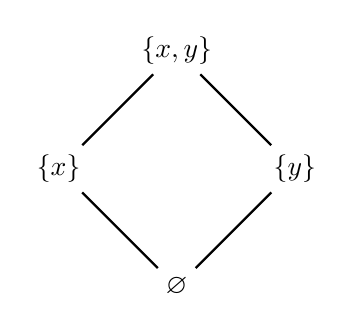
\begin{tikzpicture}[scale=1.5]

  % poset
  \draw (-1cm,0cm) node (v2) {$\{x\}$};
  \draw (1cm,0cm)  node (v3) { $\{y\}$ };
  \draw (0cm,-1cm) node (v4) {$\varnothing$};
  \draw (0cm,1cm)  node (v1) {$\{x,y\}$};

  \draw[thick]  (v1) edge (v2);
  \draw[thick]  (v3) edge (v1);
  \draw[thick]  (v3) edge (v4);
  \draw[thick]  (v2) edge (v4);

  \end{tikzpicture}
\end{center}
\caption{The Hasse Diagram of the poset $(P({x,y}), \subseteq)$.}
\label{fig:hasse}
\end{figure}

A poset can be represented as a Hasse diagram, as shown in the example of figure \ref{fig:hasse}.

\begin{definition}
Let $(W,S)$ be a Coxeter system and $T = \{wsw^{-1} | w \in W, s \in S\}$ a set of reflections. Two elements $u, w \in W$ define a function $u \to v$ if $l(v) > l(u)$ and $v = ut$ for some $t \in T$.
We define an order $w \leq v$ if there exists:

\begin{equation}
u \to u_1 \to u_2 \to \dots \to u_k = v
\end{equation}
\end{definition}
A Bruhat order is a partial order on the elements of a Coxeter group. By using the relation defined in the previous definition, we can have a Bruhat order as shown in figure \ref{fig:bruhat}.

\begin{figure}
\begin{center}

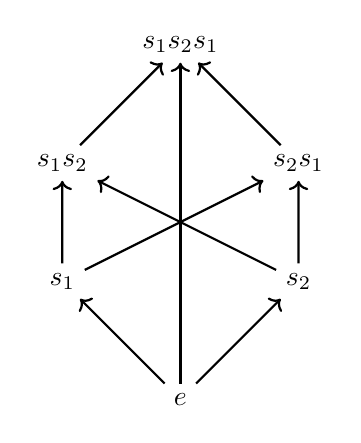
\begin{tikzpicture}[scale=1.5]

  % poset
  \draw (-1cm,0cm) node (v2) {$s_1$};
  \draw (1cm,0cm)  node (v3) {$s_2$ };
  \draw (0cm,-1cm) node (v4) {$e$};
  \draw (-1cm,1cm)  node (v1) {$s_1s_2$};
  \draw (1cm,1cm)  node (v5) {$s_2s_1$};
  \draw (0cm,2cm)  node (v6) {$s_1s_2s_1$};

  \draw[<-, thick]  (v1) edge (v2);
  \draw[->, thick]  (v2) edge (v5);
  \draw[->, thick]  (v3) edge (v1);
  \draw[<-, thick]  (v3) edge (v4);
  \draw[<-, thick]  (v2) edge (v4);
  \draw[->, thick]  (v3) edge (v5);
  \draw[->, thick]  (v1) edge (v6);
  \draw[->, thick]  (v5) edge (v6);
  \draw[->, thick]  (v4) edge (v6);

\end{tikzpicture}
\end{center}
\caption{The Bruhat order $(S_3, \{s_1, s_2\}), T = \{s_1,s_2,s_3,s_4,s_5\}$}
\label{fig:bruhat}
\end{figure}


\begin{theorem}
  Let $u,v \in S_n$, $u \leq v$ if and only if the intersection degree of $u$ is $\leq$ than the one of $v$.
\end{theorem}

\begin{example}
  If we have $35124 \leq 45213$:
  \begin{equation}
    \begin{split}
      3 &\leq 4\\
      35 &\leq 45\\
      135 &\leq 245\\
      1235 &\leq 1245\\
      12345 &\leq 12345
    \end{split}
  \end{equation}
\end{example}

\begin{theorem} [Subword property]
  Let $v = s_1s_2\dots s_q$ reduced word for $v \in W$. Then $u \leq v$ if and only if $u = s_{i_1}s_{i_2} \dots s_{i_k}$ reduced for some $1 \leq i_1 \leq i_2 \leq \dots \leq i_k \leq q$.
\end{theorem}

\begin{proof}
We first prove the \emph{if} part of the theorem. Assume $u \to v$, so $v = ut$ and $l(v) > l(u) = l(utt) = l(vt)$ for some $t \in T$.
By the exchange property:
\begin{equation}
u = vt = s_1s_2\dots \hat{s_i} \dots s_q
\end{equation}
We omit factors iteratively until we have what we want.\\
Second, we prove the \emph{only if} part of the theorem by induction on $l(v) - l(u)$.
If $l(v)-l(u) = 1$ and we have
\begin{equation}
  u = s_1 \dots \hat{s_i} \dots s_q
\end{equation}
with
\begin{equation}
  t = s_q \dots s_i \dots s_q
\end{equation} then $ut = v$ which means that $u \to v$.
If $l(v) - l(u) > 1$ and we have
\begin{equation}
  u = s_1 \dots \hat{s_{a_1}} \dots \hat{s_{a_2}} \dots \hat{s_{a_k}} \dots s_q
\end{equation}
with a minimal $k$ such that $l(v) - l(u) = k$, we take
\begin{equation}
  t = s_q \dots s_{a_k} \dots s_q
\end{equation}
and
\begin{equation}
  ut = s_1 \dots \hat{s_{a_1}} \dots \hat{s_{a_2}} \dots s_{a_k} \dots s_q
\end{equation}
We could have two cases:
\begin{itemize}
  \item Case $l(ut) > l(u)$: \\
  then $l(ut) = l(u) +1$, so $u \to ut$. $l(v)-l(ut) -1$. By induction $ut \leq v$, so $u \leq v$.
  \item Case $l(ut) < l(u)$: \\
 this will be proved impossible by contradiction. By exchange we have
  \begin{equation}
    ut = s_1 \dots \hat{s_{a_1}} \dots \hat{s_{i}} \dots \hat{s_{a_{k-1}}} \dots s_{a_{k}} \dots s_q
  \end{equation}
  If $i > a_k$ and we have
  \begin{equation}
    t = s_q \dots s_1 \dots s_q
  \end{equation}
Then,
  \begin{equation}
    \begin{split}
      vtt &= s_1 \dots s_q (s_q \dots s_{a_k} \dots s_q)(s_q \dots s_i \dots s_q)\\
      &= s_q \dots \hat{s_{a_k}} \dots \hat{s_i} \dots s_q
    \end{split}
  \end{equation}
  which is a contradiction.\\

  If $i < a_k$,
  \begin{equation}
    \begin{split}
      u = utt &= s_1 \dots \hat{s_{a_1}} \dots s_q (s_q \dots \hat{s_{a_k}} \dots s_i \dots \hat{s_k} \dots s_q) (s_q \dots s_{a_k} \dots{s_q})\\
      &= s_1 \dots \hat{s_{a_1}} \dots \hat{s_i} \dots s_{a_k} \dots s_q
    \end{split}
  \end{equation}
You can see that we omit elements to the left of $a_k$, which contradicts the minimality of $a_k$. This proves that the case when $l(ut) < l(u)$ is impossible. Thus, we have proved the first case true which finishes the proof. \qed

\end{itemize}
\end{proof}

From this theorem we can deduct some corollaries.

\begin{corollary}
  $u \leq v$ if and only if $u^{-1} \leq v^{-1}$.
\end{corollary}

\begin{corollary}
  If $u \leq v$ and $l(v) - l(u) = k$, then
  \begin{equation}
    u \leq u_1 \leq u_2 \leq \dots \leq u_k
  \end{equation}
  with $l(u_i) = l(u) + i$ for every $i$.
\end{corollary}

\begin{proof}
Let $v = s_1 \dots s_q$ and $l(v) = q$, $u \leq v$, $l(v) - l(u) = k$ so $l(u) = q-k$. By subword property

\begin{equation}
  u_1 = s_i \dots \hat{s_{a_k}} \dots s_q = u\underset{t}{\underbrace{s_q \dots s_{a_k} \dots s_q}}
\end{equation}
We have then $l(u_1) = l(ut) = l(u)+1$, so $u \to u_1$ which means that $u \leq u_1$. \qed
\end{proof}

\begin{theorem}[Lifting property]
  If $u, v \in W$ and $s \in S$ with $u \leq w$, then $u \leq sw$ and $su \leq w$.
\end{theorem}
\begin{proof}
Take $sw = s_1 \dots s_q$ in a reduced form.
Since $sw \leq w$, $w = ss_1\dots s_q$ is also reduced.
As $u \leq w$, $u$ is a subword of $ss_1 \dots s_q$. If $u$ is a subword of $s_1 \dots s_q$, this corresponds to the theorem. If not,
\begin{equation}
  u = ss_{i_1} \dots s_{i_r}
\end{equation}
is reduced with
\begin{equation}
  1 \leq i_1 \leq i_2 \leq \dots \leq i_r \leq q
\end{equation}
So $su = s_{i_1} \dots s_{i_2}$, which is a contradiction as $u \leq su$. The proof of $su \leq w$ is left to the reader. \qed
\end{proof}

\begin{lemma}
  If $u,v \in W$ then it exists a $w \in W$ such that $u \leq w$ and $v \leq w$.
\end{lemma}

\begin{proof}
  We can prove this by induction on $l(u) + l(v)$. Say $l(u) > 0$:

  We take $s \in S$ such that $l(su)= l(u) - 1$. By induction $l(su) + l(v) < l(u) + l(v)$ so it exists indeed a $w \in W$ such that $su \leq w$ and $v \leq w$. We may have two different cases: if $sw \leq w$ or $w \leq sw$:

  \begin{itemize}
    \item Case $w \leq sw$: by the lifting property, $v \leq sw$ and $u \leq sw$.
    \item Case $sw \leq w$: again by the lifting property, $v \leq w$ and $u \leq w$.
  \end{itemize}

  This proves that there always exists an element that respects the lemma, either $w$ or $sw$. \qed
\end{proof}

\begin{corollary}
If $W$ is finite, there is an unique maximal $w_0 \in W$.
\end{corollary}

\begin{example}
  In $S_n$ we have $w_0 = n(n-1) \dots 1$.
\end{example}

\begin{corollary}
  If there is a $w_0 \in W$ such that $sw_0 \leq w_0$ for all $s \in S$, then $w \leq w_0$ for all $w \in W$ and $W$ is finite.
\end{corollary}

\begin{proof}
  The proof is left to the reader. You may prove this by induction on $l(w)$, by showing that $w \leq w_0$ for all $w \in W$. Then show finitely many choices of $w$.
\end{proof}

This maximal element is very important because it has some properties that relates it with the set of reflections $T$:

\begin{proposition}
  Let $w_0 \in W$ be the maximal element of $W$ and $T_L(w) = \{t\in T |\  l(tw) < l(w)\}$. The following statements are true:
  \begin{itemize}
    \item $w_0^2 = e$
    \item $l(ww_0) = l(w_0) - l(w)$
    \item $T_L(ww_0) = T \setminus T_L(w_0)$
    \item $l(w_0) = |T|$
  \end{itemize}
\end{proposition}

\begin{corollary}
  $u \leq v$ if and only if $vw_0 \leq uw_0$.
\end{corollary}


\backmatter%%%%%%%%%%%%%%%%%%%%%%%%%%%%%%%%%%%%%%%%%%%%%%%%%%%%%%%
%%%%%%%%%%%%%%%%%%%%%%%% referenc.tex %%%%%%%%%%%%%%%%%%%%%%%%%%%%%%
% sample references
% "computer science"
%
% Use this file as a template for your own input.
%
%%%%%%%%%%%%%%%%%%%%%%%% Springer-Verlag %%%%%%%%%%%%%%%%%%%%%%%%%%

%
% BibTeX users please use
\bibliographystyle{alpha}
\bibliography{main}
%

\printindex

%%%%%%%%%%%%%%%%%%%%%%%%%%%%%%%%%%%%%%%%%%%%%%%%%%%%%%%%%%%%%%%%%%%%%%

\end{document}
